\section{Zielsetzung}
Ziel des Versuchs ist die Bestimmung der Zusammensetzung eines Würfels, der sich aus 27 Einheitswürfeln verschiedener Materialien zusammensetzt.
Dazu wird als bildgebendes Verfahren Tomographie verwendet.


\section{Theorie}
\subsection{Grundlagen}
Als $\gamma$-Strahlungsquelle wird ${}^{137}Cs$ verwendet, dessen radioaktiver Zerfall zu ${}^{137}Ba$ in Abbildung \ref{fig:zerfall} dargestellt ist.
Das ${}^{137}Cs$ zerfällt nur mit einer Wahrscheinlichkeit von $\SI{5.4}{\%}$ direkt in den Grundzustand des ${}^{137}Ba$ und zerfällt sonst erst
in einen angeregten Bariumkern, welcher dann unter Aussendung eines Photons mit einer Energie von $\SI{0.662}{keV}$ in den Grundzustand fällt.

\begin{figure}
  \centering
  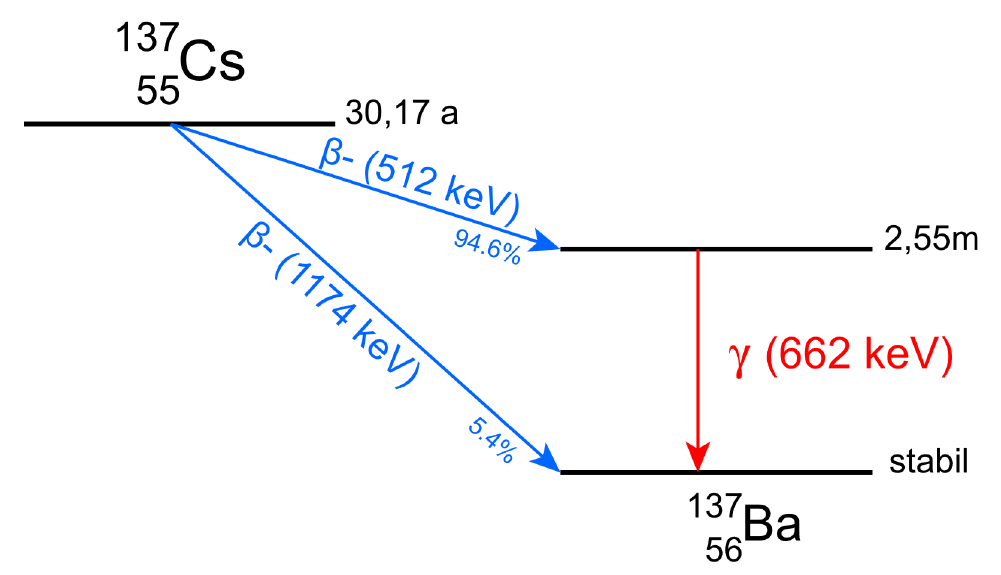
\includegraphics[scale=0.4]{graphics/Zerfall.png}
  \caption{Zerfallsschema von ${}^{137}Cs$}
  \label{fig:zerfall}
\end{figure}

Die Wechselwirkung der $\gamma$-Strahlung setzt sich im Wesentlichen aus drei verschiedenen Prozessen zusammen: Photoeffekt, Compton-Effekt und Paarbildung.
Beim Photoeffekt gibt das Photon seine gesamte Energie an ein Hüllenelektron eines Atoms ab und wird dabei ausgelöscht. Das Elektron wird dabei aus seiner
Bindung gelöst und erhält die gesamte Photonenenergie abzüglich der Bindungsenergie. Deshalb tritt der Effekt erst bei $E_\gamma > E_\text{B}$ auf.
Der Compton-Effekt beschreibt die inelastische Streuung eines Photons an einem Elektron, bei der das Photon nur einen Teil seiner Energie abgibt und nicht
ausgelöscht wird. Bis zu einer Photonenenergie von $\SI{100}{keV}$ dominiert der Photoeffekt und im Bereich $\SI{100}{keV} - \SI{10}{MeV}$ der
Compton-Effekt. Die Paarbildung tritt erst ab einer Energie von $2m_\text{e}c^2 = \SI{1.02}{MeV}$ auf, da dabei ein Photon im Coulomb-Feld eines Atomkerns
in ein Elektron und ein Positron zerfällt. Da die im Versuch verwendete Strahlung eine geringere Energie besitzt, spielt die Paarbildung hier keine Rolle.

Durch Überlagerung der verschiedenen Effekte entsteht insgesamt ein exponentieller Zusammenhang zwischen der Intensität der Strahlung und dem
Absorptionskoeffizient $\mu$ des jeweiligen Materials, welches die Strahlung durchdringt:
\begin{equation}
  N = I_0 \exp\left( \sum_i \mu_i d_i \right)
  \label{eq:N}
\end{equation}
Dabei ist $N$ die abgeschwächte Intensität, $I_0$ die Anfangintensität und die $d_i$ die Dicke des Materials in Strahlrichtung.

\subsection{Bestimmung der Absorptionskoeffizienten}
Nach Umstellen der Gleichung \eqref{eq:N} zu
\begin{equation}
  \sum_i\mu_i d_i = \ln\left(\frac{I_0}{N_j}\right)
\end{equation}
lässt sich diese in Matrixform schreiben:
\begin{equation}
  A\cdot\vec{\mu} = \vec{I}
\end{equation}
Der Vektor $\vec{\mu}$ enthält dabei sämtliche Absorptionskoeffizienten der Elementarwürfel und der Vektor $\vec{I}$ die Anfangsintensität und die jeweiligen abgeschwächten
Intensitäten für die verschiedenen gewählten Strahlengänge. Die Matrix $A$ enthält die Informationen über die Abstände. Da eine Schicht des Würfels aus
neun Elementarwürfeln besteht, ist die Matrix für $m$ Messungen $9\times m$-dimensional. Damit das Gleichungssystem lösbar ist, müssen mindestens 9
Messungen gemacht werden. Da der Würfel jedoch nicht ganz exakt im Strahlengang ausgerichtet werden kann, werden mehr Messungen vorgenommen, sodass ein
überbestimmtes Gleichungssystem entsteht. Abbildung \ref{fig:wuerfel} zeigt die ausgewählten Projektionen.

\begin{figure}
  \centering
  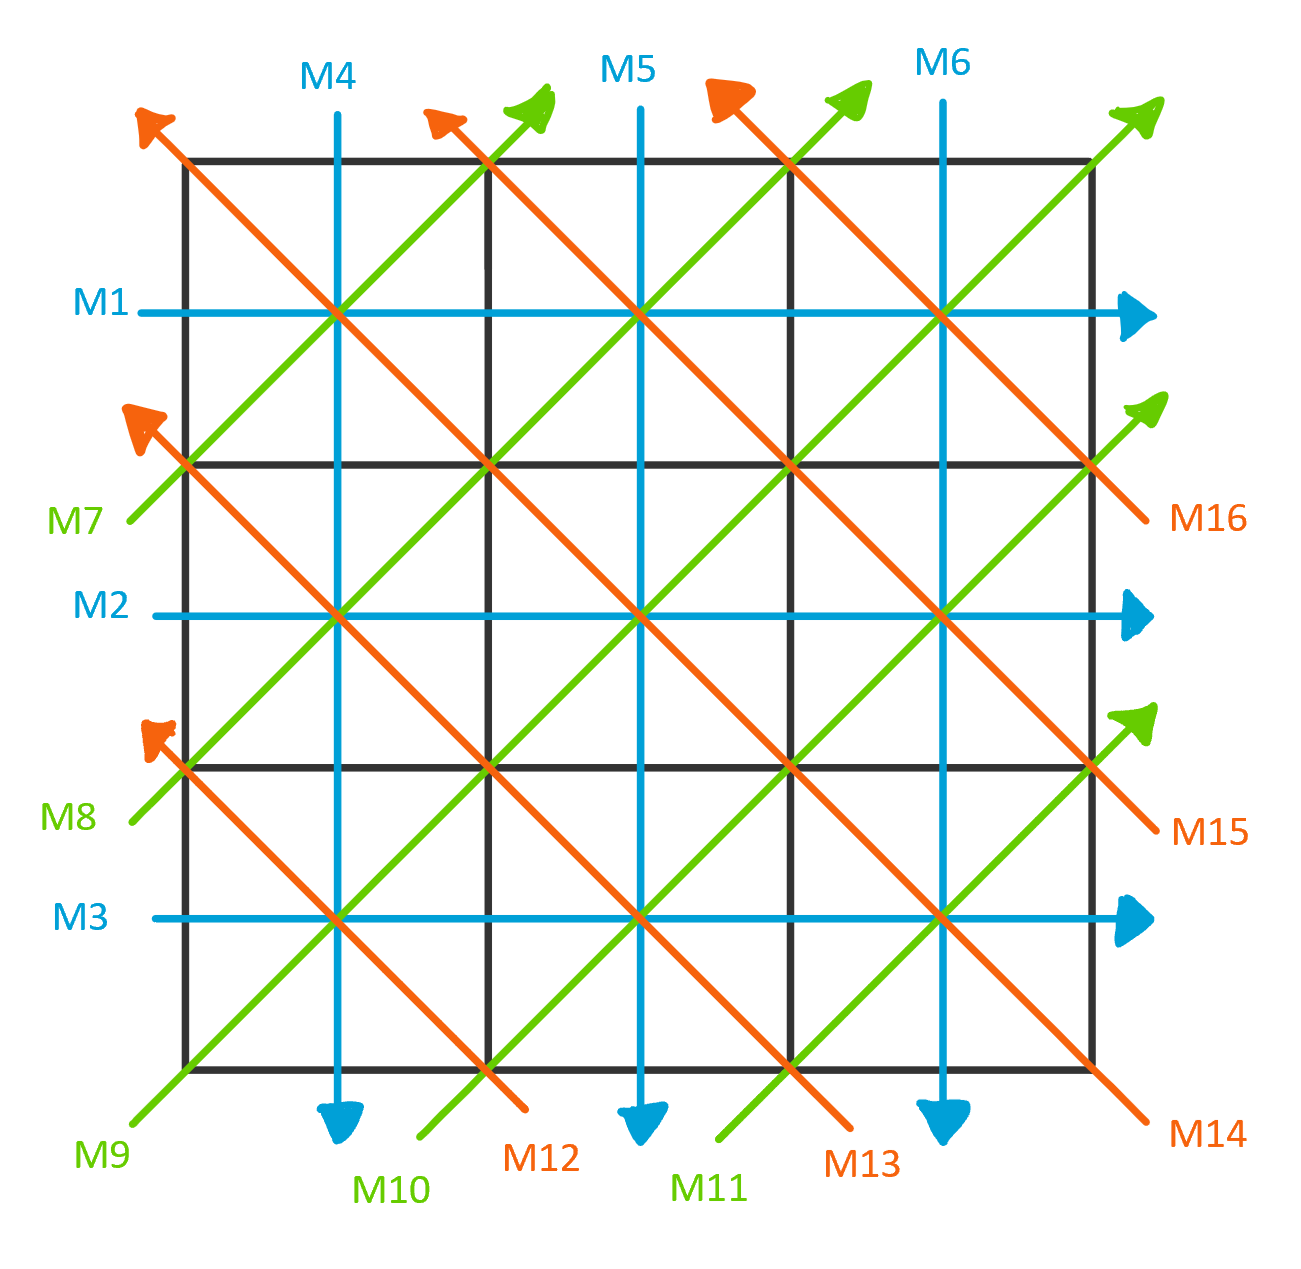
\includegraphics[scale=0.5]{graphics/wuerfel.png}
  \caption{Die ausgewählten Projektionen zur Messung der mittleren Schicht eines 3x3x3 Würfels.}
  \label{fig:wuerfel}
\end{figure}
